%%
%% This is file `sample-manuscript.tex',
%% generated with the docstrip utility.
%%
%% The original source files were:
%%
%% samples.dtx  (with options: `manuscript')
%% 
%% IMPORTANT NOTICE:
%% 
%% For the copyright see the source file.
%% 
%% Any modified versions of this file must be renamed
%% with new filenames distinct from sample-manuscript.tex.
%% 
%% For distribution of the original source see the terms
%% for copying and modification in the file samples.dtx.
%% 
%% This generated file may be distributed as long as the
%% original source files, as listed above, are part of the
%% same distribution. (The sources need not necessarily be
%% in the same archive or directory.)
%%
%% Commands for TeXCount
%TC:macro \cite [option:text,text]
%TC:macro \citep [option:text,text]
%TC:macro \citet [option:text,text]
%TC:envir table 0 1
%TC:envir table* 0 1
%TC:envir tabular [ignore] word
%TC:envir displaymath 0 word
%TC:envir math 0 word
%TC:envir comment 0 0
%%
%%
%% The first command in your LaTeX source must be the \documentclass command.
\documentclass[manuscript,screen,review,nonacm]{acmart}
\usepackage{hyperref,xurl}
%%
%% \BibTeX command to typeset BibTeX logo in the docs
\AtBeginDocument{%
  \providecommand\BibTeX{{%
    \normalfont B\kern-0.5em{\scshape i\kern-0.25em b}\kern-0.8em\TeX}}}

%% Rights management information.  This information is sent to you
%% when you complete the rights form.  These commands have SAMPLE
%% values in them; it is your responsibility as an author to replace
%% the commands and values with those provided to you when you
%% complete the rights form.
% \setcopyright{acmcopyright}
% \copyrightyear{2018}
% \acmYear{2018}
% \acmDOI{XXXXXXX.XXXXXXX}

%% These commands are for a PROCEEDINGS abstract or paper.
% \acmConference[CS 235]{Data Mining Techniques}{Fall 2023}{University of California, Riverside}
% \acmPrice{15.00}
% \acmISBN{978-1-4503-XXXX-X/18/06}


%%
%% Submission ID.
%% Use this when submitting an article to a sponsored event. You'll
%% receive a unique submission ID from the organizers
%% of the event, and this ID should be used as the parameter to this command.
%%\acmSubmissionID{123-A56-BU3}

%%
%% For managing citations, it is recommended to use bibliography
%% files in BibTeX format.
%%
%% You can then either use BibTeX with the ACM-Reference-Format style,
%% or BibLaTeX with the acmnumeric or acmauthoryear sytles, that include
%% support for advanced citation of software artefact from the
%% biblatex-software package, also separately available on CTAN.
%%
%% Look at the sample-*-biblatex.tex files for templates showcasing
%% the biblatex styles.
%%

%%
%% The majority of ACM publications use numbered citations and
%% references.  The command \citestyle{authoryear} switches to the
%% "author year" style.
%%
%% If you are preparing content for an event
%% sponsored by ACM SIGGRAPH, you must use the "author year" style of
%% citations and references.
%% Uncommenting
%% the next command will enable that style.
%%\citestyle{acmauthoryear}

%%
%% end of the preamble, start of the body of the document source.
\begin{document}

%%
%% The "title" command has an optional parameter,
%% allowing the author to define a "short title" to be used in page headers.
\title{CS235 Fall'23 Project Midterm Report}
%%
%% The "author" command and its associated commands are used to define
%% the authors and their affiliations.
%% Of note is the shared affiliation of the first two authors, and the
%% "authornote" and "authornotemark" commands
%% used to denote shared contribution to the research.
% \author{Ben Trovato}
% \authornote{Both authors contributed equally to this research.}
% \email{trovato@corporation.com}
% \orcid{1234-5678-9012}
% \author{G.K.M. Tobin}
% \authornotemark[1]
% \email{webmaster@marysville-ohio.com}
% \affiliation{%
%   \institution{Institute for Clarity in Documentation}
%   \streetaddress{P.O. Box 1212}
%   \city{Dublin}
%   \state{Ohio}
%   \country{USA}
%   \postcode{43017-6221}
% }

\author{Liam Y. Hsieh (lhsie013)}
\affiliation{
  \institution{University of California, Riverside}
  \streetaddress{900 University Ave}
  \city{Riverside}
  \country{U.S.A}}
\email{liam.hsieh@email.ucr.edu}
\authorsaddresses{}
% \author{Valerie B\'eranger}
% \affiliation{%
%   \institution{Inria Paris-Rocquencourt}
%   \city{Rocquencourt}
%   \country{France}
% }

% \author{Aparna Patel}
% \affiliation{%
%  \institution{Rajiv Gandhi University}
%  \streetaddress{Rono-Hills}
%  \city{Doimukh}
%  \state{Arunachal Pradesh}
%  \country{India}}

% \author{Huifen Chan}
% \affiliation{%
%   \institution{Tsinghua University}
%   \streetaddress{30 Shuangqing Rd}
%   \city{Haidian Qu}
%   \state{Beijing Shi}
%   \country{China}}

% \author{Charles Palmer}
% \affiliation{%
%   \institution{Palmer Research Laboratories}
%   \streetaddress{8600 Datapoint Drive}
%   \city{San Antonio}
%   \state{Texas}
%   \country{USA}
%   \postcode{78229}}
% \email{cpalmer@prl.com}

% \author{John Smith}
% \affiliation{%
%   \institution{The Th{\o}rv{\"a}ld Group}
%   \streetaddress{1 Th{\o}rv{\"a}ld Circle}
%   \city{Hekla}
%   \country{Iceland}}
% \email{jsmith@affiliation.org}

% \author{Julius P. Kumquat}
% \affiliation{%
%   \institution{The Kumquat Consortium}
%   \city{New York}
%   \country{USA}}
% \email{jpkumquat@consortium.net}

%%
%% By default, the full list of authors will be used in the page
%% headers. Often, this list is too long, and will overlap
%% other information printed in the page headers. This command allows
%% the author to define a more concise list
%% of authors' names for this purpose.
%\renewcommand{\shortauthors}{Liam Y. Hsieh}

%%
%% The abstract is a short summary of the work to be presented in the
%% article.
\begin{abstract}
This project focuses on predicting car sales prices using Deep Learning and compares them to a baseline linear regression model. The dataset, obtained from Kaggle, comprises 500 records with features like customer demographics and financial information. The ANN model is structured with an input layer, two hidden layers using ReLU activation, and an output layer for regression. Evaluation employs Mean Absolute Error (MAE) as the primary metric. Liam Hsieh is the sole contributor for this project, aiming to optimize predictive accuracy and provide valuable insights for the automotive industry.
\end{abstract}

%%
%% Keywords. The author(s) should pick words that accurately describe
%% the work being presented. Separate the keywords with commas.
\keywords{Car sales price prediction, Deep Learning, Neural Networks, Mean Absolute Error (MAE)}


%%
%% This command processes the author and affiliation and title
%% information and builds the first part of the formatted document.
\maketitle

\section{Current State}
\urldef{\repourl}\url{https://github.com/liam-hsieh/CS235/tree/main/project/code}
The code for this project can be found at GitHub\footnote{\repourl}.
The high-level flow for proposed approach is shown as Fig. \ref{fig:flowchart}.   

\begin{figure}
  \centering
  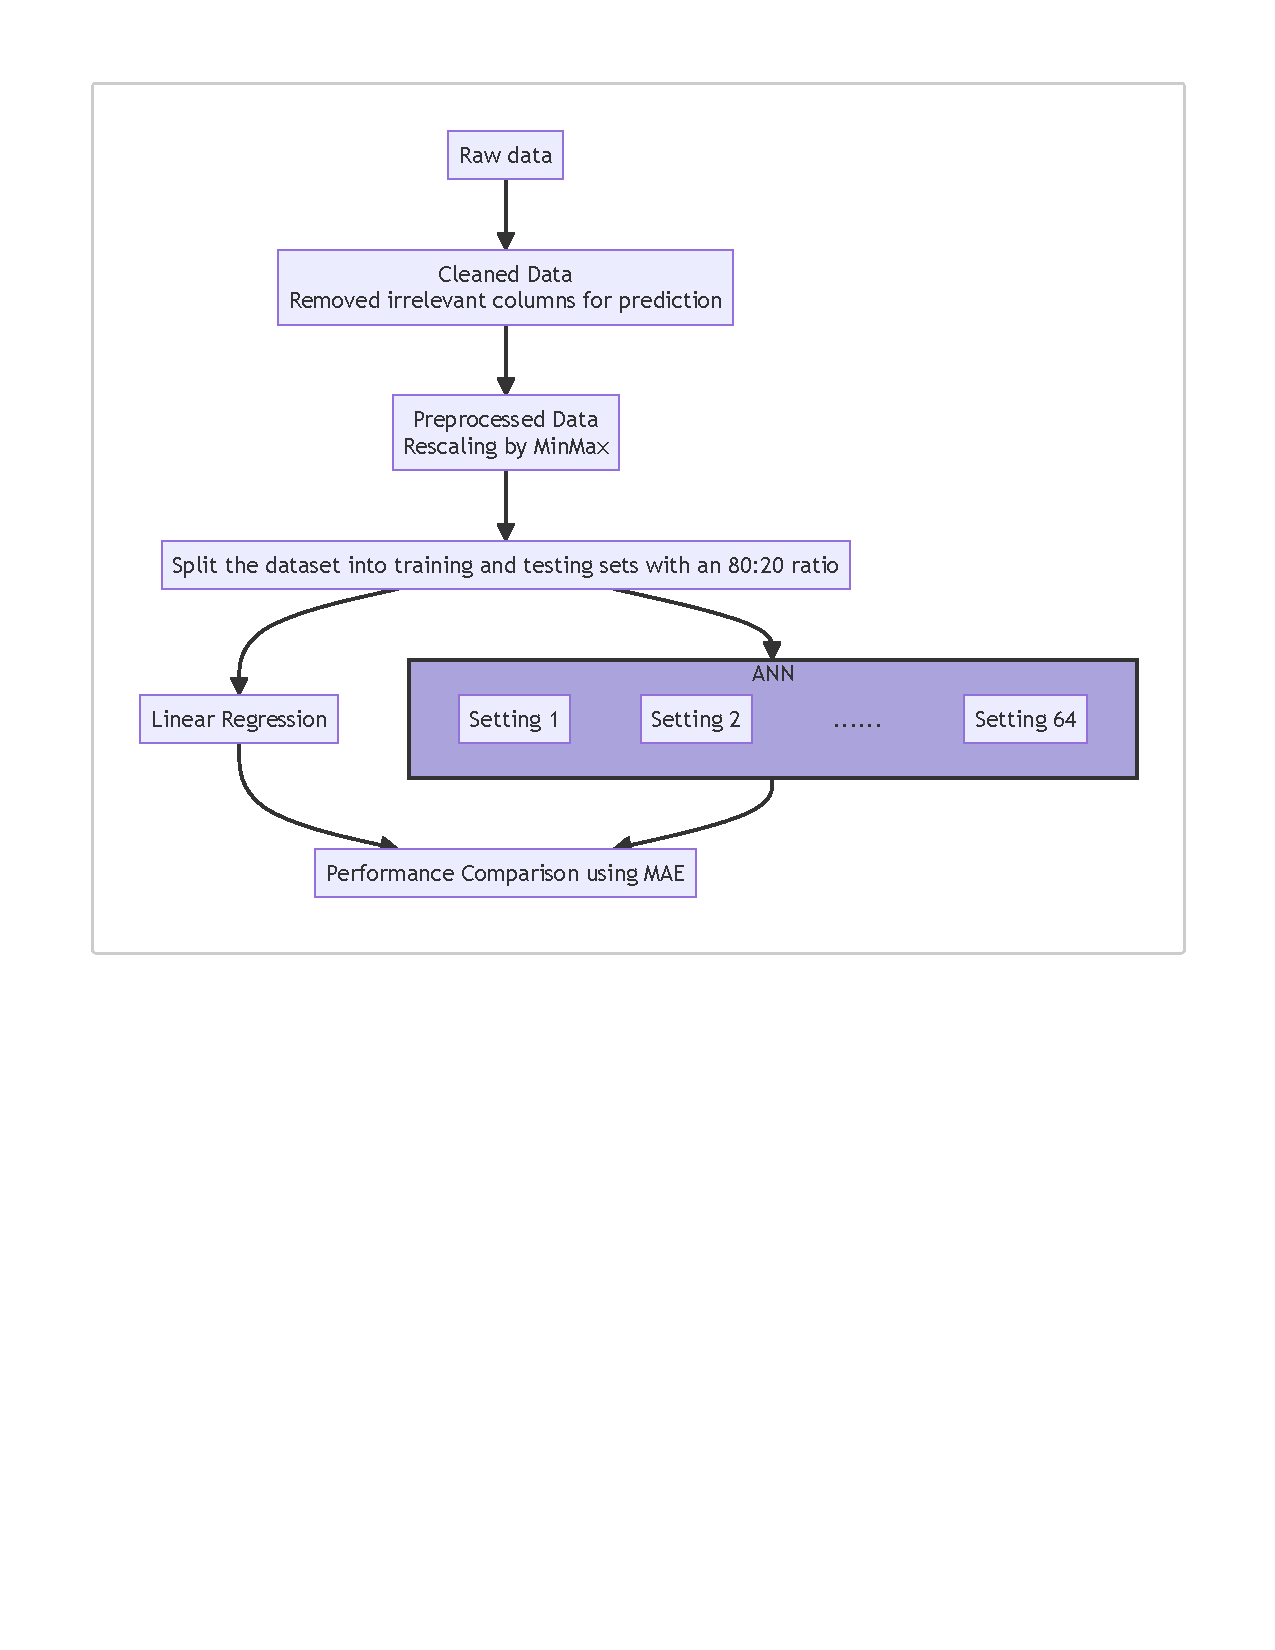
\includegraphics[width=0.8\linewidth]{flowchart.pdf}
  \caption{Project Overview.}
  \label{fig:flowchart}
\end{figure}

BRIEFLY EXPLAIN the flow

More details on performance comparison

\subsection{Artificial Neuron Network}
In the project proposal, we mentioned the method would be used and different settings are investigated. 

In this project, we systematically investigate the performance of different ANN structures and optimization methods to identify the optimal configuration for predicting our target variable. We consider a range of activation functions, including 'relu,' 'tanh,' 'sigmoid,' and 'linear,' and vary the number of neurons in each layer with choices of 8, 16, 32, and 64 neurons. Additionally, we explore different optimizers, such as 'adam,' 'sgd,' 'rmsprop,' and 'adagrad.'

We generate ANN models based on the combinations of activation functions, neuron counts, and optimizers. Each model consists of multiple layers, including an input layer with 5 dimensions, hidden layers with the specified number of neurons and chosen activation function, and an output layer with a linear activation function. All models are compiled using the mean squared error loss function and mean absolute error as the evaluation metric.

For each model, we train it on a training set (X_train, y_train) for 50 epochs with a validation split of 20\%. We collect performance metrics, mean absolute error, during training for both the training and validation sets. These metrics provide insights into how well each configuration performs on the given dataset.

The experiment aims to analyze and compare the performance of these different configurations, helping us identify the most suitable ANN architecture and optimization strategy for our predictive modeling task.

\section{PRELIMINARY RESULTS}
Accurately predicting car sales prices is a critical task that significantly influences purchasing decisions for both consumers and dealerships. The existing methods often rely on traditional statistical approaches like linear regression, which may not fully capture the complexities and non-linearity present in the data. The problem at hand involves utilizing Artificial Neural Networks (ANNs), a powerful tool in machine learning, to predict car sales prices. ANN models can potentially grasp intricate patterns and relationships within the dataset, enabling superior predictive performance compared to conventional linear regression methods. By exploring different ANN architectures and comparing them with a baseline linear regression model, we aim to identify the most effective approach for predicting car sales prices accurately.

\subsection{Dataset}
\urldef{\dataurl}\url{https://www.kaggle.com/datasets/yashpaloswal/ann-car-sales-price-prediction}


The dataset utilized in this project is sourced from Kaggle \footnote{\dataurl} and is centered around predicting car sales prices using machine learning techniques. The dataset contains 500 records with 9 columns, featuring both predictors and the target variable. 


\textbf{Predictors}:
\begin{itemize}
    \item Customer Name: The name of the customer.
    \item Customer Email: The email address of the customer.
    \item Country: The country of the customer.
    \item Gender: Gender of the customer (binary encoding: 0 for male, 1 for female).
    \item Age: Age of the customer.
    \item Annual Salary: The customer's annual salary.
    \item Credit Card Debt: The amount of credit card debt the customer has.
    \item Net Worth: The net worth of the customer.
\end{itemize}

\textbf{Target/Label}:
\begin{itemize}
    \item Car Purchase Amount: The amount a customer spends on purchasing a car.
\end{itemize}


The dataset provides a diverse range of customer information that can be utilized to train and evaluate machine learning models for predicting car purchase amounts. The inclusion of both demographic and financial features allows for a comprehensive analysis, which is crucial in building accurate prediction models for car sales prices. 

\section{Proposed Approach}
The proposed approach involves initially splitting the dataset into a training set (80\%) and a testing set (20\%). The core of the project revolves around leveraging Artificial Neural Networks (ANNs) to predict car sales prices. The ANN architecture comprises an input layer representing selected features, two hidden layers activated using Rectified Linear Unit (ReLU) functions, and an output layer for regression, employing the mean squared error loss. The Keras library, built on TensorFlow, will be utilized to implement the ANN model. Specifically, the output layer will employ a linear activation function to predict numeric car purchase amounts. Different activation functions will be explored and compared to determine the most effective model configuration. The ANN model will be compiled using a defined optimizer and loss function, and subsequently trained on the training set. Evaluation of the ANN's performance will be conducted using the testing set. Additionally, a baseline linear regression model will be implemented and compared with the ANN model to assess and compare predictive performances, ultimately selecting the most accurate and efficient model for car sales price prediction.


\section{Evaluation Metrics}
For assessing the accuracy of our car sales price prediction models, Mean Absolute Error (MAE) will be the primary evaluation metric. MAE calculates the average absolute differences between the predicted and actual car purchase amounts. A lower MAE signifies a more accurate prediction model, where smaller absolute differences indicate closer alignment between predicted and observed prices. 

 

\end{document}
\endinput
%%
%% End of file `sample-manuscript.tex'.
